\chapter{پیاده‌سازی سیستم}

در این قسمت نحوه‌ی اجرای پروژه را بطور کامل توضیح خواهیم داد. در هر قسمت ساختار فایل‌ها، نحوه‌ی پیاده‌سازی و چالش‌هایی که با آن مواجه بودیم به‌همراه نحوه‌ی حل آنها را توضیح خواهیم داد.

\section{معماری کلی سیستم}

برای درک بهتر این پروژه، نمایی کلی از سیستم و نحوه عملکرد آن را همانطور که در \cref{fig:system_overview} نشان داده شده است، ارائه خواهیم داد. این پروژه در چندین محل صنعتی مستقر خواهد شد. در هر کارخانه چندین میکروکنترلر آردوینو، با یک سنسور لرزش و یک فرستنده گیرنده زیگبی متصل، روی هر قطعه از تجهیزات نصب شده است. داده‌ها در زمان‌های برنامه‌ریزی‌شده حس می‌شوند و سپس به دروازه‌ای در کارخانه ارسال می‌شوند. دروازه اطلاعاتی را که از فرستنده‌گیرنده‌های زیگبی می‌آید را جمع‌آوری می‌کند تا زمانی که به یک آستانه‌ی از پیش تعریف‌شده برسد. سپس دروازه با سرور مرکزی احراز هویت می‌شود و سپس داده‌های جمع‌آوری‌شده را با پروتکل \lr{HTTP} به سرور ارسال می‌کند. در سرور مراحل پیش‌پردازش لازم انجام می‌شود و سپس داده‌ها در پایگاه داده‌ی سری زمانی ذخیره می‌شوند. سپس مدل یادگیری ماشین با داده‌های قبلی و جدید اجرا می‌شود تا پیش‌بینی دقیق‌تری درباره طول عمر مفید باقیمانده تجهیزات به ما ارائه دهد. در صورت درخواست، تمام داده‌های تحلیلی و پیشبینی‌ها از طریق داشبورد مدیریت قابل‌دسترسی است. متخصصان می‌توانند از این داده‌ها برای برنامه‌ریزی زمان نگهداری مناسب استفاده کنند.

\begin{figure}[!h]
\centering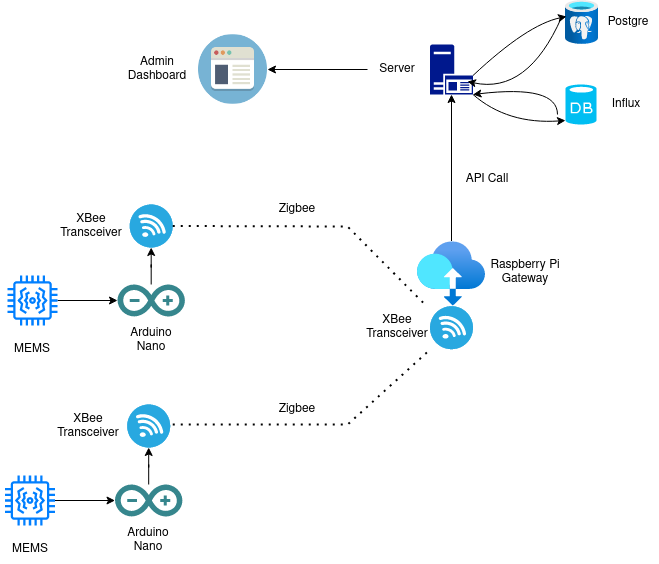
\includegraphics[scale=.6]{system_overview.png}
\caption{نمای کلی سیستم}\label{fig:system_overview}
\end{figure}

\section{گره انتهایی و آردوینو}

برای پیاده‌سازی گره انتهایی، سه بخش را باید پیاده‌سازی میکردیم که عبارتند از:

\begin{itemize}
\item خواندن از حسگر و نمونه‌برداری
\item تشکیل فریم زیگبی و نوشتن در درگاه سریال
\item خوابیدن و بیدارشدن در بازه‌های زمانی مشخص
\end{itemize}

در ادامه هر بخش را توضیح می‌دهیم.

\subsection{خواندن از حسگر و نمونه‌برداری}

حسگر \lr{ADXL345} چندین پارامتر دارد که باید در زمان راه‌اندازی تنظیم شوند. برای انجام پیکربندی و همچنین خواندن داده‌های حسگرها بدون نیاز به استفاده مستقیم از پروتکل \lr{I2C}، از کتابخانه\LTRfootnote{Adafruit\_ADXL345\_U.h} استفاده کرده‌ایم. یکی از پارامترها محدوده شتاب است که با تابع \lr{setRange} تنظیم می‌شود. محدوده مجاز ۲، ۴، ۸ یا ۱۶ برابر شتاب گرانش زمین است. اما هرچه دامنه بزرگتر شود، داده‌ها دقت کمتری پیدا می‌کنند. از آنجایی که یک قطعه از تجهیزات حتی زمانی که قدیمی باشد با شتاب بالا نمی‌لرزد و برای پیش‌بینی‌های دقیق‌تر به دقت نیاز است، تصمیم گرفتیم که محدوده را روی دو برابر شتاب گرانش زمین تنظیم کنیم.


پارامتر دیگر نرخ داده است که باید در زمان راه‌اندازی با استفاده از تابع \lr{setDataRate} تنظیم شود. نرخ داده برای تنظیم نرخ ارتباط بین حسگر و بورد آردوینو از طریق پروتکل \lr{I2C} استفاده می‌شود. بنابراین مهم است که نرخ داده با رسانه‌ی ارتباطی سازگار باشد. از آنجایی که اگر نرخ داده بالاتر از نرخی باشد که رسانه قادر به انجام آن است، برخی از داده‌ها از بین می‌روند. بدلیل برخی چالش‌های دیگر که در ادامه در مورد آنها صحبت خواهد شد، نرخ را روی ۱۰۰ هرتز تنظیم کرده‌ایم. برای نمونه‌برداری از داده‌ها در فرکانس نمونه‌برداری مورد نظر، تأخیر نمونه‌برداری برای تأخیر بین هر نمونه حسگر محاسبه می‌شود.

برای هر نمونه، از یک رویداد برای بدست‌آوردن شتاب در سه محور \lr{x}، \lr{y}، \lr{z} استفاده می‌کنیم. سپس داده‌ها در یک آرایه ذخیره می‌شوند تا بعداً قالب‌بندی و با پروتکل زیگبی ارسال شوند. اگر فرمت و ارسال در حین نمونه‌برداری انجام شود، بدلیل تاخیر در فرمت، تشکیل و ارسال فریم‌ها از طریق درگاه سریال، فرکانس نمونه‌برداری صحیح نخواهد بود.

ما چالش دیگری در این شرایط بوجود می‌آید. با توجه به محدودیت حافظه موجود در دستگاه آردوینو نانو، فضای ایجاد آرایه‌ها و ذخیره داده‌ها نیز محدود است. به همین دلیل است که نمی‌توانیم به فرکانس‌های نمونه‌برداری بالا دست پیدا کنیم.

\subsection{تشکیل فریم زیگبی و نوشتن در درگاه سریال}

همانطور که در \cref{sub:xbee} گفته شد، در حالت شفاف پیام‌ها به‌شکل مستقیم منتقل می‌شوند اما در حالت \lr{API} نیاز به تشکیل فریم دارند. ابتدا سراغ استفاده از کتابخانه‌های آماده برای تشکیل و نوشتن فریم بر روی درگاه سریال رفتیم. یکی از آنها کتابخانه \lr{xbee-arduino}\LTRfootnote{\url{https://github.com/andrewrapp/xbee-arduino}} بود. اما این کتابخانه مشکلات فراوانی داشت که سبب عدم ارسال فریم توسط ماژول می‌شد. یکی از این مشکلات محاسبه اشتباه چک‌سام و عدم مطابقت با استاندارد بود. مشکل دیگر نیز در نوشتن بر روی درگاه سریال بود. همه این مشکلات باعث شد تا ما کتابخانه خود را پیاده‌سازی کنیم. اگرچه این پیاده‌سازی کلی نیست و بعضا برای این پروژه انجام شده است، اما کارکرد مورد انتظار را دارد.

\subsubsection{کتابخانه \lr{Xbee}}

ساختار فایل کتابخانه ایکس‌بی در \cref{fig:xbee_lib} نشان داده شده است. ساختار طبق استانداردهای آردوینو\LTRfootnote{\url{https://arduino.github.io/arduino-cli/0.33/library-specification/}} برای ایجاد یک کتابخانه است. فایل‌های اصلی در پوشه \lr{src} قرار دارند، یک فایل هدر که توابع، ورودی‌ها و خروجی‌ها را تعریف می‌کند و یک فایل سی‌پلاس‌پلاس برای پیاده‌سازی و تکمیل آن توابع. در پوشه نمونه‌ها، فایلی با فرمت \lr{ino} وجود دارد که کاربرد اصلی کتابخانه برای انتقال یک فریم در حالت \lr{API} را نشان می‌دهد. یک فایل \lr{library.properties} در ریشه پوشه وجود دارد. این فایل برای تشریح برخی از ویژگی‌های این کتابخانه از جمله نام، نویسنده، توضیحات، نسخه کتابخانه، معماری‌های سازگار و اینکه این کتابخانه به کدام کتابخانه‌ها وابستگی دارد استفاده می‌شود. این فایل به \lr{IDE} آردوینو کمک می‌کند تا کتابخانه و وابستگی‌های آن را نصب کند.

\begin{figure}[!h]
\centering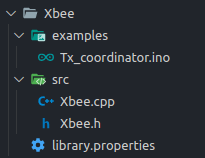
\includegraphics[scale=1]{xbee_lib.png}
\caption{ساختار فایل کتابخانه ایکس‌بی}\label{fig:xbee_lib}
\end{figure}

\subsubsection{ساختار فریم \lr{API}}

ساختار کلی فریم \lr{API} در \cref{fig:xbee_frame} \cite{Digi} نشان داده شده است. فریم با یک بایت جداکننده شروع می‌شود، سپس با ۲ بایت برای نشان‌دادن طول فریم ادامه می‌یابد و با یک بایت چک‌سام پایان می‌یابد. بایت‌های بین طول و فیلد چک‌سام را داده‌های فریم می‌نامند که برای هر نوع بسته \lr{API} متفاوت است. بایت اول فیلد طول مهم‌ترین بایت\LTRfootnote{Most Significant Byte(MSB)} و بایت بعدی کم‌اهمیت‌ترین\LTRfootnote{Least Significant Byte(LSB)} است. اولین بایت از داده‌های فریم نشان‌دهنده نوع فریم است. چک‌سام برای کمک به تست یکپارچگی داده‌ها استفاده می‌شود. اگر مقدار چک‌سام به اشتباه محاسبه شده‌باشد یا با چک‌سام واقعی داده‌های درون فریم متفاوت باشد، فریم کنار گذاشته و نادیده گرفته می‌شود.


\begin{figure}[!h]
\centering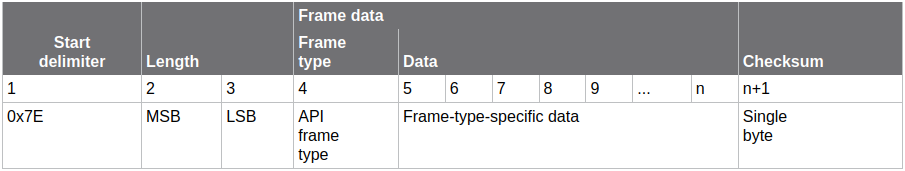
\includegraphics[scale=.65]{xbee_frame.png}
\caption{ساختار کلی فریم \lr{API} \cite{Digi}}\label{fig:xbee_frame}
\end{figure}

روش صحیح محاسبه چک‌سام فریم به شرح زیر است:
\begin{enumerate}
\item تمام بایت‌های بسته به استثنای محدودکننده شروع و طول با هم جمع می‌شوند.
\item از نتیجه فقط پایین‌ترین ۸ بیت نگه داشته می‌شود.
\item مقدار بدست‌آمده از \lr{0xFF} کم می‌شود.
\end{enumerate}

\subsubsection{فریم درخواست ارسال} \label{tx_req}

فریم‌های \lr{API} بسته به عملکردشان از چندین نوع فریم پشتیبانی می‌کنند. در این بخش فقط در مورد فریم درخواست ارسال که برای ما مهم است صحبت خواهیم کرد.

بخش‌های مختلف داده‌های فریم درخواست ارسال در \cref{tab:tx_req_frame} به همراه کاربرد آمده است.

\begin{table}[h!]
  \begin{center}
    \caption{بخش‌های مختلف داده‌های فریم درخواست ارسال \cite{Digi}}
    \label{tab:tx_req_frame}
    \begin{tabular}{|p{.1\textwidth}|p{.1\textwidth}|p{.25\textwidth}|p{.45\textwidth}|} % <-- Alignments: 1st column left, 2nd middle and 3rd right, with vertical lines in between
	   	\hline
	   	نام بخش & شماره بایت & نمونه & توضیحات\\
		\hline
	   	نوع فریم & ۳ & \lr{0x10} & بایت \lr{0x10} نشان‌دهنده فریم درخواست ارسال است.\\
		\hline
	   		   	شماره فریم & ۴ & \lr{0x01} & فریم داده را به گیرنده برای ارسال فریم وضعیت ارسال می‌شناساند. تنظیم‌کردن با مقدار ۰ پاسخ را غیرفعال می‌کند.\\
	    \hline
	   	آدرس ۶۴ بیتی مقصد & ۵ تا ۱۲ & \lr{0x0000000000000000} & آدرس ۶۴ بیتی مقصد را مشخص می‌کند.
	   	
 آدرس مقاصد خاص:
 
 	   	هماهنگ‌کننده: \lr{0x0000000000000000}
 	   	
همه‌پخشی\LTRfootnote{Broadcast}: \lr{0x000000000000FFFF}  	

نامعلوم(اگر آدرس مقصد را ندانیم): \lr{0xFFFFFFFFFFFFFFFF}
	   	\\
		\hline
	   	 	آدرس ۱۶ بیتی مقصد & ۵ تا ۱۲ & \lr{0x0000} & آدرس ۱۶ بیتی مقصد را مشخص می‌کند.
	   	
 آدرس مقاصد خاص:
 
 	   	هماهنگ‌کننده: \lr{0x0000}
 	   	

نامعلوم یا همه‌پخشی: \lr{0xFFFE}
	   	\\
		\hline
		شعاع پخش & ۱۵ & \lr{0x00} & حداکثر تعداد پرش‌هایی که انتقال همه‌پخشی می‌تواند پخش شود را تنظیم می‌کند. اگر روی ۰ تنظیم شود، شعاع پخش روی حداکثر مقدار پرش تنظیم می‌شود.\\
		\hline
		انتخاب‌ها & ۱۶ & \lr{0x00} & گزینه‌های انتقال پشتیبانی‌شده:

غیرفعال‌کردن تلاش ارسال مجدد - \lr{0x01}		

فعال‌کردن رمزگذاری \lr{APS}(با این کار حداکثر بایت‌های داده ارسالی تا ۴ بایت کاهش می‌یابد) - \lr{0x20}

استفاده از مهلت زمان طولانی برای ارسال - \lr{0x40}
		\\
		\hline
		داده ارسالی & ۱۷ به بعد & \lr{0x...} & تا ۲۵۵ بایت داده ارسالی برای مقصد\\
    	\hline
    \end{tabular}
  \end{center}
\end{table}

\subsubsection{داده ارسالی}

برای استفاده بهینه از فضای پیام در هر فریم، تصمیم گرفتیم ارتعاشات حسگر را به صورت زیر ارسال کنیم:

\begin{itemize}
\item هر داده با دقت ۳ رقم اعشار ارسال می‌شود.
\item برای جداسازی ارتعاش بر اساس محور در پیام ارسالی، از حروف \lr{x}، \lr{y} و \lr{z} استفاده نمی‌کنیم.
\item اولین بایت همیشه شناسه اندازه‌گیری را نشان می‌دهد. پس از آن پنج بایت اول نشان‌دهنده محور ایکس، پنج بایت بعدی نشان‌دهنده محور وای و پنج بایت بعدی نشان‌دهنده محور زد است. هر داده در پنج بایت نمایش داده می‌شود، برای مثال عدد ۴۵۲/۳- بصورت \lr{\{'-','3','4','5','2'\}} نمایش داده می‌شود.
\end{itemize}

در سمت گیرنده، داده‌ها باید به حالت اولیه تبدیل شوند.

\subsubsection{فایل \lr{Xbee.cpp} و توابع مهم}

برای تنظیم آدرس مقصد برای هر فریم کلاس \lr{XbeeDestAddress} را تعریف کرده‌ایم. این کلاس شامل فیلد ۶۴ بیتی و ۱۶ بیتی برای آدرس است. با توجه به اینکه به آرایه‌ای از بایت‌ها برای تشکیل فریم نیاز داریم، توابعی متناظر برای گرفتن هر یک از فیلدها نیز نوشته شده است.


برای تشکیل فریم درخواست انتقال کلاس \lr{XbeeRequest} تعریف شده است. تابع \lr{constructFrame} برای ایجاد فریم با استفاده از شناسه فریم و داده مورد نظر نوشته شده است. این تابع فریم را طبق \cref{tx_req} ایجاد کزده و فریم تشکیل‌شده برگردانده می‌شود. با استفاده از تابع \lr{writeFrameToSerial} نیز می‌توان فریم تشکیل‌شده را بر روی درگاه سریال دلخواه نوشت.

\subsection{‫ﺧﻮﺍﺑﻴﺪﻥ‬ ‫ﻭ‬ ‫ﺑﻴﺪﺍﺭﺷﺪﻥ‬ ‫ﺩﺭ‬ ‫ﺑﺎﺯﻩ‬‌‫ﻫﺎی ‬‫ﺯﻣﺎﻧﻲ‬ ‫ﻣﺸﺨﺺ‬}

برای کاهش مصرف انرژی، حسگر تنها در زمان‌های مشخص لرزش را احساس می‌کند. در سایر زمان‌ها بورد آردوینو برای کاهش مصرف انرژی به خواب می‌رود. برای این کار از کتابخانه \lr{LowPower.h} استفاده می‌کنیم. با استفاده از تابع \lr{powerDown} آردوینو به خواب می‌رود. برای بیدارشدن در زمان مشخص، آردوینو از زمان‌بند داخلی خود\LTRfootnote{Watchdog Timer} استفاده می‌کند. اما این تایمر بعد از ۸ ثانیه سرریز شده و بورد بیدار می‌شود. برای زمان‌های بیشتر باید به محض بیدارشدن مجدد تا رسیدن به زمان مورد نظر، آن را مجددا به خواب ببریم. این کار در تابع \lr{longSleep} انجام شده است.

\section{دروازه}

در دروازه ما از زبان برنامه‌نویسی پایتون برای دریافت فریم‌های زیگبی، ذخیره‌کردن و ارسال داده‌ها به سرور مرکزی پس از رسیدن به آستانه استفاده می‌کنیم. ساختار پروژه دروازه در \cref{fig:gateway_structure} نشان داده شده است. در این بخش به بررسی هر یک از فایل ها می‌پردازیم.


\begin{figure}[!h]
\centering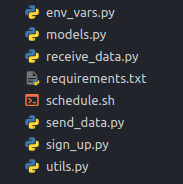
\includegraphics[scale=1]{gateway_structure.png}
\caption{ساختار پروژه دروازه}\label{fig:gateway_structure}
\end{figure}

\subsection{فایل \lr{env\_vars.py}}

این فایل از بسته \lr{load\_dotenv} برای خواندن متغیرهای محیطی استفاده می‌کند. برخی از این متغیرها برای برقراری ارتباط با سرور استفاده می‌شوند مانند شماره پورت سرور و آیپی سرور. سایر آنها برای برقراری ارتباط با دستگاه ایکس‌بی استفاده می‌شوند. این متغیرهای محیطی به عنوان متغیرهای پایتون تنظیم می‌شوند و سپس در ماژول‌های دیگر پایتون استفاده می‌شوند.

\subsection{فایل \lr{models.py}}

در این فایل ما سه کلاس برای نمایش داده‌های ارتعاش، اندازه گیری‌ها و هر گره انتهایی تعریف کرده‌ایم.

کلاس داده ارتعاش شامل داده‌های لرزش در سه محور ثبت‌شده توسط حسگر می‌باشد. هر اندازه‌گیری بسته به فرکانس نمونه‌برداری شامل چندین داده ارتعاش است. همچنین شامل یک شناسه و زمانی است که اندازه‌گیری در آن انجام شده است. از آنجایی که برای برقراری ارتباط داده‌های ارتعاش با زیگبی قطعه‌بندی\LTRfootnote{Fragmentation} لازم است و زمانی بین ارسال هر فریم لازم است، تابع \lr{thread\_handler} تعریف شده است تا در صورت اتمام زمان اتصال یا از بین رفتن برخی فریم‌ها، اندازه‌گیری از داده‌های دریافتی قبلی بطور خودکار تکمیل شود. پس از آن داده‌های جدید ذخیره می‌شوند.

هر گره دارای یک شناسه است که با شناسه فرستنده ارائه‌شده در هر فریم زیگبی مشخص می‌شود. همچنین هر گره شامل چندین اندازه‌گیری است. هنگامی که اندازه‌گیری جدیدی به لیست اندازه‌گیری‌ها اضافه می‌شود، زمان‌بند رشته‌ای\LTRfootnote{Thread Timer} با دوره وقفه مشخص و تابع \lr{thread\_handler} شروع می‌شود.

\subsection{فایل \lr{receiver.py}}

در این فایل سروری تعریف می‌کنیم که بطور بی‌نهایت به درگاه \lr{USB} متصل به دستگاه ایکس‌بی گوش می‌دهد. برای خواندن داده‌ها و استخراج داده هر فریم از کتابخانه \lr{digi-xbee} استفاده می‌کنیم. برای مقداردهی اولیه یک نمونه ایکس‌بی، درگاه و نرخ باود\LTRfootnote{Buad Rate} ارتباط لازم است. در تابع \lr{decode\_sensor\_data}، شناسه اندازه‌گیری و داده‌های ارتعاش را استخراج می‌کنیم. در تابع \lr{receive}، به منتظر دریافت پیام جدید می‌مانیم. داده‌های پیام را به گره و اندازه‌گیری مربوطه اضافه می‌کنیم و سپس داده‌های ذخیره‌شده را بروز می‌کنیم.

\subsection{فایل \lr{requirements.txt}}

این فایل برای تعیین بسته‌ها، نسخه‌ها و وابستگی‌های لازم استفاده می‌شود. سپس از این فایل برای نصب بسته‌های مشخص‌شده با مدیریت بسته پایتون پیپ\LTRfootnote{pip} استفاده می‌شود.

\subsection{فایل \lr{schedule.sh}}

آستانه تعریف‌شده بر اساس زمان است. این اسکریپت در کنار گیرنده اجرا می‌شود. در این اسکریپت یک کار \lr{crontab} برنامه‌ریزی می‌شود که هر ۱۵ دقیقه اجرا شود. این زمان‌بندی با استفاده از علامت \lr{*/15 * * * *} انجام می‌شود که به معنای اجرای اسکریپت ارسال داده پایتون در هر دقیقه قابل‌تقسیم بر ۱۵ است.

\subsection{فایل \lr{send\_data.py}}

در این فایل اطلاعات ذخیره‌شده در حافظه بارگذاری می‌شود. برای سرور و فراخوانی نقاط انتهایی \lr{API} از کتابخانه \lr{requests} استفاده می‌کنیم. برای دریافت رمز احراز هویت \lr{JWT} برای ارسال داده‌های ارتعاشی، یک درخواست پست با آدرس مک دستگاه و رمز عبور به سرور ارسال می‌شود تا رمز احراز هویت را دریافت کند. پس از آن داده‌های لرزش فرمت‌شده بصورت جیسان\LTRfootnote{JavaScript Object Notation(JSON)} در بدنه درخواست به همراه هدر احراز هویت به سرور ارسال و فایل ذخیره نیز پاک می‌شود.

\subsection{فایل \lr{signup.py}}

این فایل برای ثبت دروازه در سرور با رمز عبور و آدرس مک مربوطه استفاده می‌شود.

\subsection{فایل \lr{utils.py}}

این فایل شامل برخی از توابع کاربردی مانند دریافت آدرس مک دستگاه، دریافت زمان جاری در شکل مورد نظر، بروز رسانی داده‌های ذخیره‌شده و تعریف کلاس مدل جیسان برای کد‌کردن داده‌ها می‌باشد.

\section{پیش‌پردازش}

داده‌های جمع‌آوری‌شده از حسگر در هر سه محور می‌توانند تحت تاثیر شتاب گرانش زمین باشند. همچنین شتاب اندازه‌گیری‌شده توسط حسگرهای کم‌هزینه \lr{MEMS} نیز اکثرا تحت تاثیریک مقدار غیرصفر دچار انحرافاتی می‌شوند که منجر به افزایش یا کاهش اندازه‌گیری‌ها می‌شود\cite{jung2017vibration}. برای حذف انحرافات و شتاب گرانش ناخواسته، داده‌ها را در مرحله پیش‌پردازش هنجارسازی می‌کنیم. برای حذف ناهنجاری‌ها مطابق \cref{form:norm} میانگین هر محور را ار هر داده کم می‌کنیم. لازم به ذکر است که $\hat{a}^l_{nm}$ نماد ماتریس هنجارشده برای شتاب در سه محور، گره \lr{n} و اندازه‌گیری \lr{m}ام است.

\begin{equation}
\label{form:norm}
\hat{a}^l_{nm}=a^l_{nm}-\sum_{k=1}^K \dfrac{a^l_{nmk}}{K}
\end{equation}

\section{پایگاه داده سری زمانی}




